% Options for packages loaded elsewhere
\PassOptionsToPackage{unicode}{hyperref}
\PassOptionsToPackage{hyphens}{url}
\documentclass[
  11pt,
  ignorenonframetext,
]{beamer}
\newif\ifbibliography
\usepackage{pgfpages}
\setbeamertemplate{caption}[numbered]
\setbeamertemplate{caption label separator}{: }
\setbeamercolor{caption name}{fg=normal text.fg}
\beamertemplatenavigationsymbolsempty
% remove section numbering
\setbeamertemplate{part page}{
  \centering
  \begin{beamercolorbox}[sep=16pt,center]{part title}
    \usebeamerfont{part title}\insertpart\par
  \end{beamercolorbox}
}
\setbeamertemplate{section page}{
  \centering
  \begin{beamercolorbox}[sep=12pt,center]{section title}
    \usebeamerfont{section title}\insertsection\par
  \end{beamercolorbox}
}
\setbeamertemplate{subsection page}{
  \centering
  \begin{beamercolorbox}[sep=8pt,center]{subsection title}
    \usebeamerfont{subsection title}\insertsubsection\par
  \end{beamercolorbox}
}
% Prevent slide breaks in the middle of a paragraph
\widowpenalties 1 10000
\raggedbottom
\AtBeginPart{
  \frame{\partpage}
}
\AtBeginSection{
  \ifbibliography
  \else
    \frame{\sectionpage}
  \fi
}
\AtBeginSubsection{
  \frame{\subsectionpage}
}
\usepackage{iftex}
\ifPDFTeX
  \usepackage[T1]{fontenc}
  \usepackage[utf8]{inputenc}
  \usepackage{textcomp} % provide euro and other symbols
\else % if luatex or xetex
  \usepackage{unicode-math} % this also loads fontspec
  \defaultfontfeatures{Scale=MatchLowercase}
  \defaultfontfeatures[\rmfamily]{Ligatures=TeX,Scale=1}
\fi
\usepackage{lmodern}
\usetheme[]{Madrid}
\ifPDFTeX\else
  % xetex/luatex font selection
\fi
% Use upquote if available, for straight quotes in verbatim environments
\IfFileExists{upquote.sty}{\usepackage{upquote}}{}
\IfFileExists{microtype.sty}{% use microtype if available
  \usepackage[]{microtype}
  \UseMicrotypeSet[protrusion]{basicmath} % disable protrusion for tt fonts
}{}
\makeatletter
\@ifundefined{KOMAClassName}{% if non-KOMA class
  \IfFileExists{parskip.sty}{%
    \usepackage{parskip}
  }{% else
    \setlength{\parindent}{0pt}
    \setlength{\parskip}{6pt plus 2pt minus 1pt}}
}{% if KOMA class
  \KOMAoptions{parskip=half}}
\makeatother
\setlength{\emergencystretch}{3em} % prevent overfull lines
\providecommand{\tightlist}{%
  \setlength{\itemsep}{0pt}\setlength{\parskip}{0pt}}
\usepackage{xcolor}
\newcommand{\hlred}[1]{\colorbox{red!20}{#1}}
\newcommand{\hlblue}[1]{\colorbox{blue!15}{#1}}
\setbeamertemplate{navigation symbols}{}
\usepackage{tikz}
\usetikzlibrary{decorations.pathreplacing}
\usepackage{subcaption}
\definecolor{targetred}{HTML}{EA5B5D}
\newcommand{\hltable}[5]{\begin{center}\begin{tikzpicture}\node[anchor=south west,inner sep=0] (img) at (0,0) {\includegraphics[width=\textwidth,height=0.78\textheight,keepaspectratio]{#1}};\begin{scope}[x={(img.south east)},y={(img.north west)}]\draw[targetred,ultra thick,fill=targetred,fill opacity=0.15] (#2,{1-#3}) rectangle ({#2+#4},{1-#3-#5});\end{scope}\end{tikzpicture}\end{center}}
\usepackage{pgfplots}
\pgfplotsset{compat=1.18}
\definecolor{curveblue}{RGB}{16, 120, 200}
\definecolor{cyangreen}{RGB}{0, 195, 160}
\definecolor{cyanfill}{RGB}{232, 252, 248}
\definecolor{pinkred}{RGB}{235, 30, 95}
\definecolor{pinkfill}{RGB}{253, 235, 243}
\definecolor{purpletext}{RGB}{125, 70, 210}
\definecolor{purplefill}{RGB}{242, 238, 255}
\usepackage{bookmark}
\IfFileExists{xurl.sty}{\usepackage{xurl}}{} % add URL line breaks if available
\urlstyle{same}
\hypersetup{
  pdftitle={PS 3: Week 13},
  pdfauthor={Maya Mikelson},
  hidelinks,
  pdfcreator={LaTeX via pandoc}}

\title{\texorpdfstring{PS 3: Week 13}{PS 3: Week 13}}
\subtitle{\texorpdfstring{Multiple Linear Regression and Experiments;
Natural
Experiments}{Multiple Linear Regression and Experiments; Natural Experiments}}
\author{\texorpdfstring{Maya Mikelson}{Maya Mikelson}}
\date{}

\begin{document}
\frame{\titlepage}

\begin{frame}{Attendance Survey}
\protect\phantomsection\label{attendance-survey}
\end{frame}

\begin{frame}{PS 3: Week 12}
\protect\phantomsection\label{ps-3-week-12}
\vspace{1.2cm}
\begin{center}
\Large Multiple Linear Regression and Experiments
\end{center}
\end{frame}

\begin{frame}{Agenda}
\protect\phantomsection\label{agenda}
\begin{enumerate}
\tightlist
\item
  Attendance Survey
\item
  MLR: Experiments
\item
  MLR: Experiments: Worksheet
\item
  Interpreting Regression Tables
\item
  Regression Table Example: Observational
\end{enumerate}
\end{frame}

\begin{frame}{Reading a Regression Table}
\protect\phantomsection\label{reading-a-regression-table}
\begin{itemize}
\tightlist
\item
  Each column reports the results of one regression. Multiple columns
  means we are looking at the results of multiple different regressions
  (in this example, two). The column titles should tell you what is
  different about the regressions. \pause

  \begin{itemize}
  \tightlist
  \item
    Sometimes this will be switching subsets of data (as in this
    example). \pause
  \item
    Sometimes it will involve switching outcomes. \pause
  \item
    Sometimes the outcome and subset will be the same, but new variables
    will be introduced into the regression. \pause
  \item
    You have to use context and the table notes to be sure what is
    changing across the columns.
  \end{itemize}
\end{itemize}
\end{frame}

\begin{frame}{Reading a Regression Table}
\protect\phantomsection\label{reading-a-regression-table-1}
\begin{itemize}
\tightlist
\item
  Each row represents the coefficients/estimates on one of the variables
  in the regression. \pause

  \begin{itemize}
  \tightlist
  \item
    The first column shows the variable that is being estimated. \pause
  \item
    The last row of estimates contains the Intercept or Constant term.
    \pause
  \item
    In each cell, the first number is the coefficient, and the number in
    brackets below it is the standard error. These are the only numbers
    we need to calculate a t-statistic, confidence interval, and
    p-value. \pause
  \item
    The stars next to each number indicate if the estimates are
    statistically significant and, if so, how small the p-value is. (The
    Table Notes along the bottom will tell you how to interpret the
    stars.)
  \end{itemize}
\end{itemize}
\end{frame}

\begin{frame}{To re-cap}
\protect\phantomsection\label{to-re-cap}
\begin{itemize}
\tightlist
\item
  Missing cells mean that this variable was not included in this
  regression. Sometimes it will just be blank, sometimes there will be a
  ``-'' to indicate it is being left blank on purpose. \pause
\item
  The sample size and R squared are printed at the bottom of each
  column. \pause
\item
  \(R^2\) or R squared is the proportion of the variation in the
  dependent variable that is predictable from the independent
  variable(s).
\end{itemize}
\end{frame}

\begin{frame}{Steps for Interpretation!}
\protect\phantomsection\label{steps-for-interpretation}
\small

\begin{enumerate}
\tightlist
\item
  Look at the \textbf{title} of the table \pause

  \begin{enumerate}
  [a.]
  \tightlist
  \item
    \textcolor{blue}{What are the authors generally trying to tell us?}
  \item
    This can clue you into relevant variables and takeaways, though keep
    a critical eye to the table yourself! \pause
  \end{enumerate}
\item
  Look at the title of each \textbf{column} (this is the title of each
  regression model) \pause

  \begin{enumerate}
  [a.]
  \tightlist
  \item
    \textcolor{blue}{What is each model trying to tell me? What subset of data are they using? What outcome?}
    \pause
  \end{enumerate}
\item
  Look at the \textbf{row} labels (these are the predictor variables)
  \pause

  \begin{enumerate}
  [a.]
  \tightlist
  \item
    \textcolor{blue}{Which ones are causal (treatment assignment)? Which ones are not (any other variables)?}
    \pause
  \end{enumerate}
\item
  Look at the point \textbf{estimates} themselves \pause

  \begin{enumerate}
  [a.]
  \tightlist
  \item
    \textcolor{blue}{Based on the row label and column title, what is this estimate telling me?}
    \pause
  \end{enumerate}
\item
  Look at the measures of \textbf{noise} \pause

  \begin{enumerate}
  [a.]
  \tightlist
  \item
    \textcolor{blue}{Is the estimate significant? How do I interpret significance in this context?}

    \begin{enumerate}
    [i.]
    \tightlist
    \item
      \textcolor{blue}{Is it causal?}
    \end{enumerate}
  \end{enumerate}
\end{enumerate}

\normalsize
\end{frame}

\begin{frame}{Table Walkthrough: Title}
\protect\phantomsection\label{table-walkthrough-title}
\begin{center}\begin{tikzpicture}\node[anchor=south west,inner sep=0] (img) at (0,0) {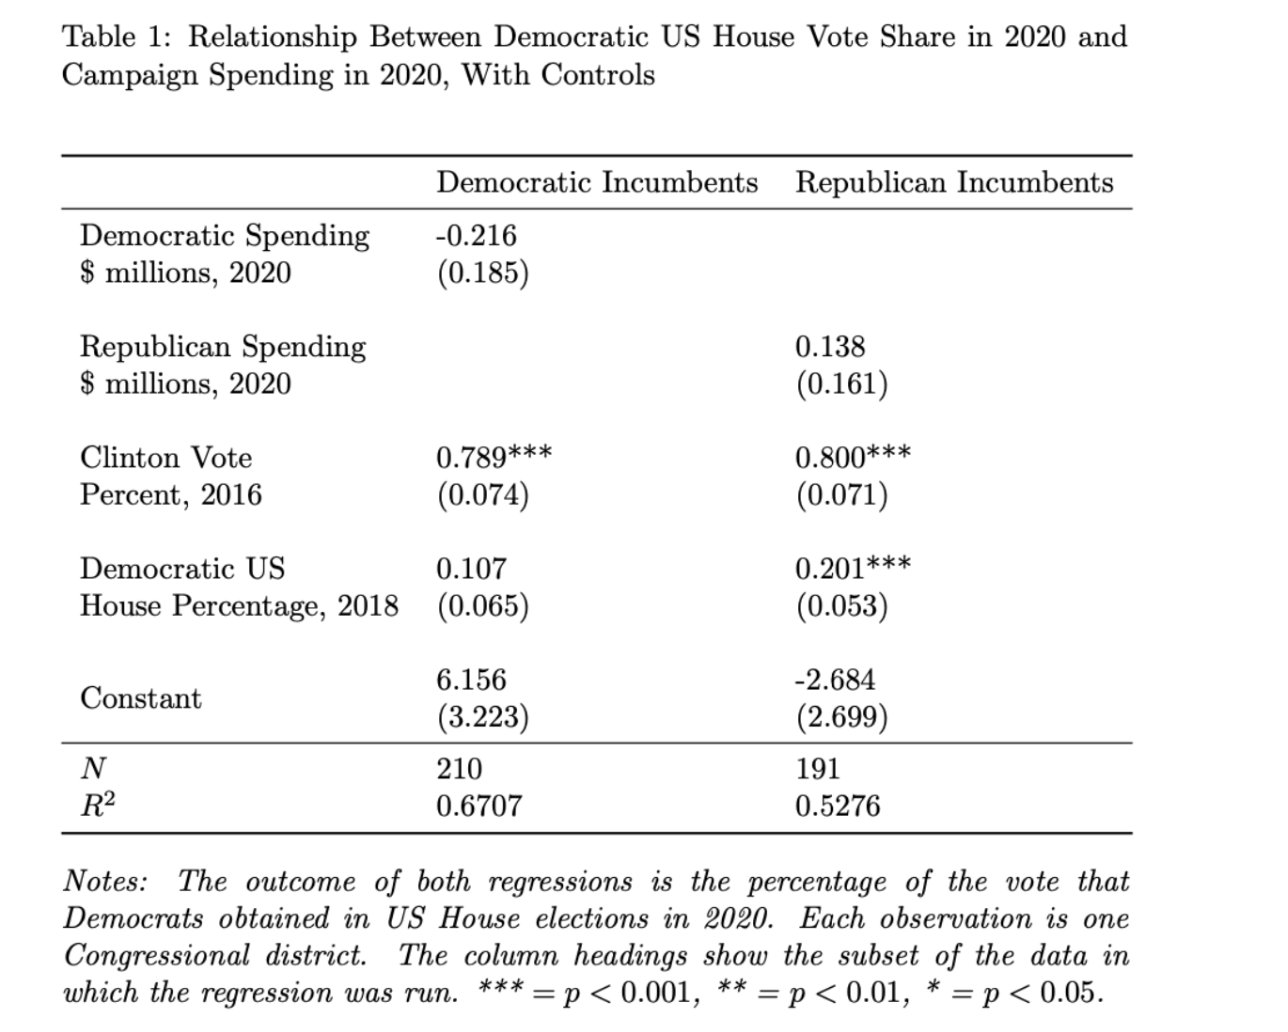
\includegraphics[width=\textwidth,height=0.78\textheight,keepaspectratio]{images/regression-table.png}};\begin{scope}[x={(img.south east)},y={(img.north west)}]\draw[targetred,ultra thick,fill=targetred,fill opacity=0.15] (0.0372,{1-0.0151}) rectangle ({0.0372+0.8622},{1-0.0151-0.0963});\end{scope}\end{tikzpicture}\end{center}
\end{frame}

\begin{frame}{Table Walkthrough: Column Titles}
\protect\phantomsection\label{table-walkthrough-column-titles}
\begin{center}\begin{tikzpicture}\node[anchor=south west,inner sep=0] (img) at (0,0) {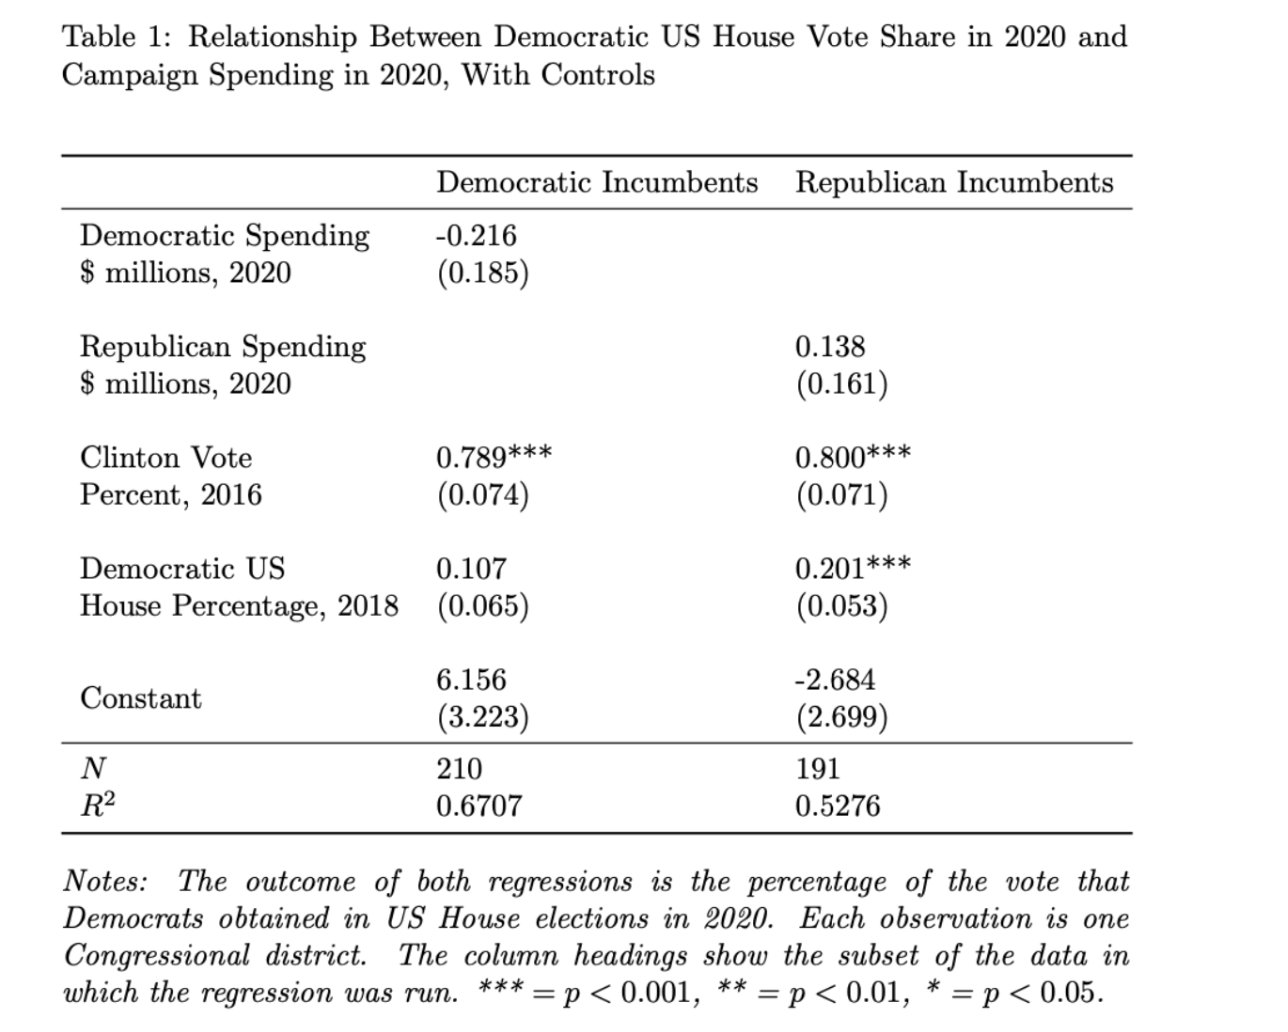
\includegraphics[width=\textwidth,height=0.78\textheight,keepaspectratio]{images/regression-table.png}};\begin{scope}[x={(img.south east)},y={(img.north west)}]\draw[targetred,ultra thick,fill=targetred,fill opacity=0.15] (0.3126,{1-0.1408}) rectangle ({0.3126+0.5932},{1-0.1408-0.0649});\end{scope}\end{tikzpicture}\end{center}
\end{frame}

\begin{frame}{Table Walkthrough: Row Labels}
\protect\phantomsection\label{table-walkthrough-row-labels}
\begin{center}\begin{tikzpicture}\node[anchor=south west,inner sep=0] (img) at (0,0) {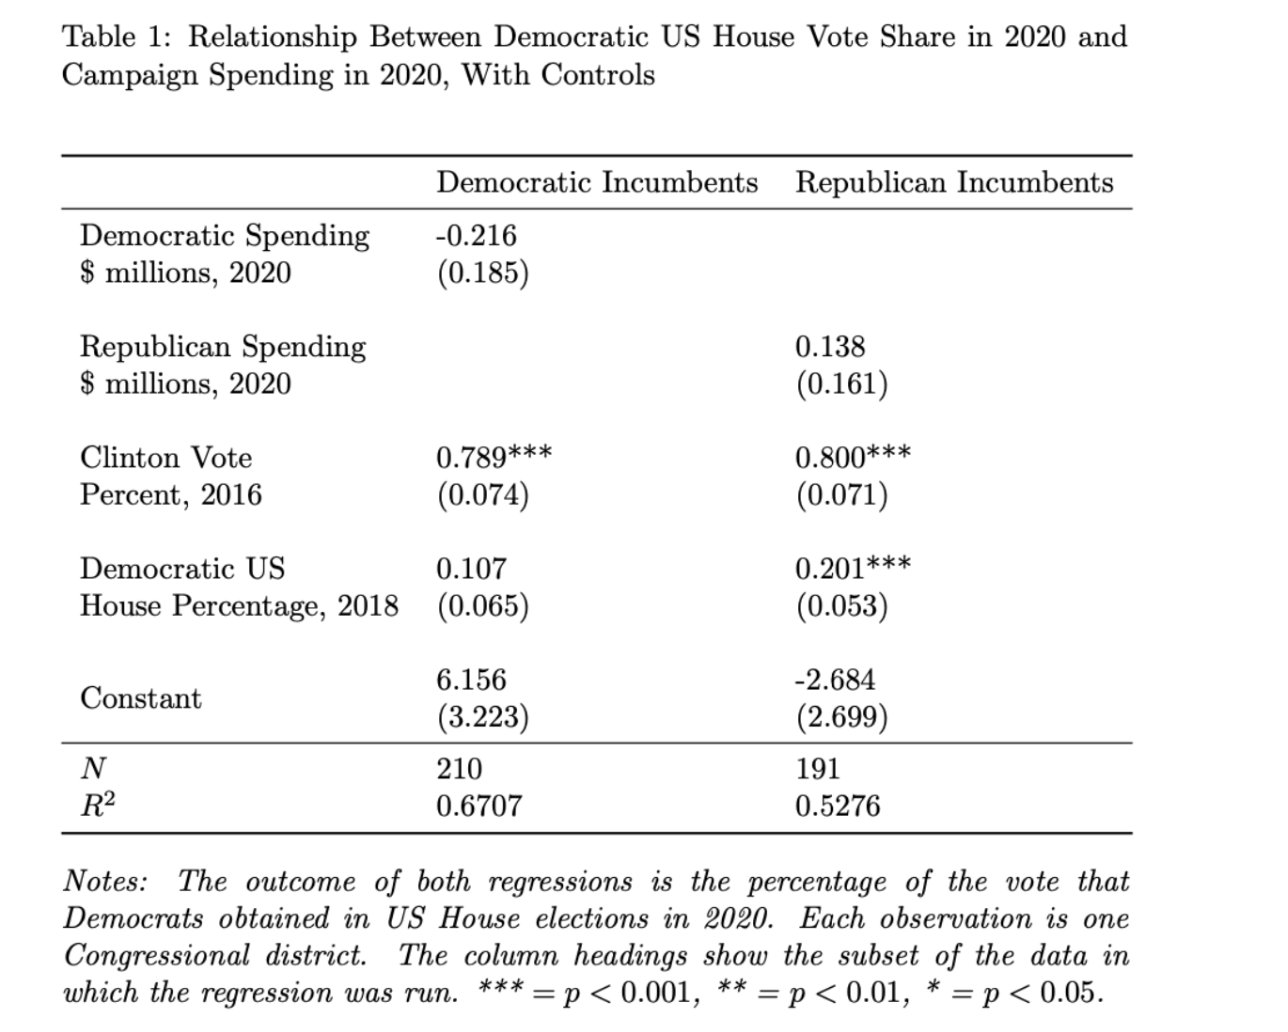
\includegraphics[width=\textwidth,height=0.78\textheight,keepaspectratio]{images/regression-table.png}};\begin{scope}[x={(img.south east)},y={(img.north west)}]\draw[targetred,ultra thick,fill=targetred,fill opacity=0.15] (0.0451,{1-0.2056}) rectangle ({0.0451+0.2801},{1-0.2056-0.5128});\end{scope}\end{tikzpicture}\end{center}
\end{frame}

\begin{frame}{Table Walkthrough: Point Estimate}
\protect\phantomsection\label{table-walkthrough-point-estimate}
\begin{center}\begin{tikzpicture}\node[anchor=south west,inner sep=0] (img) at (0,0) {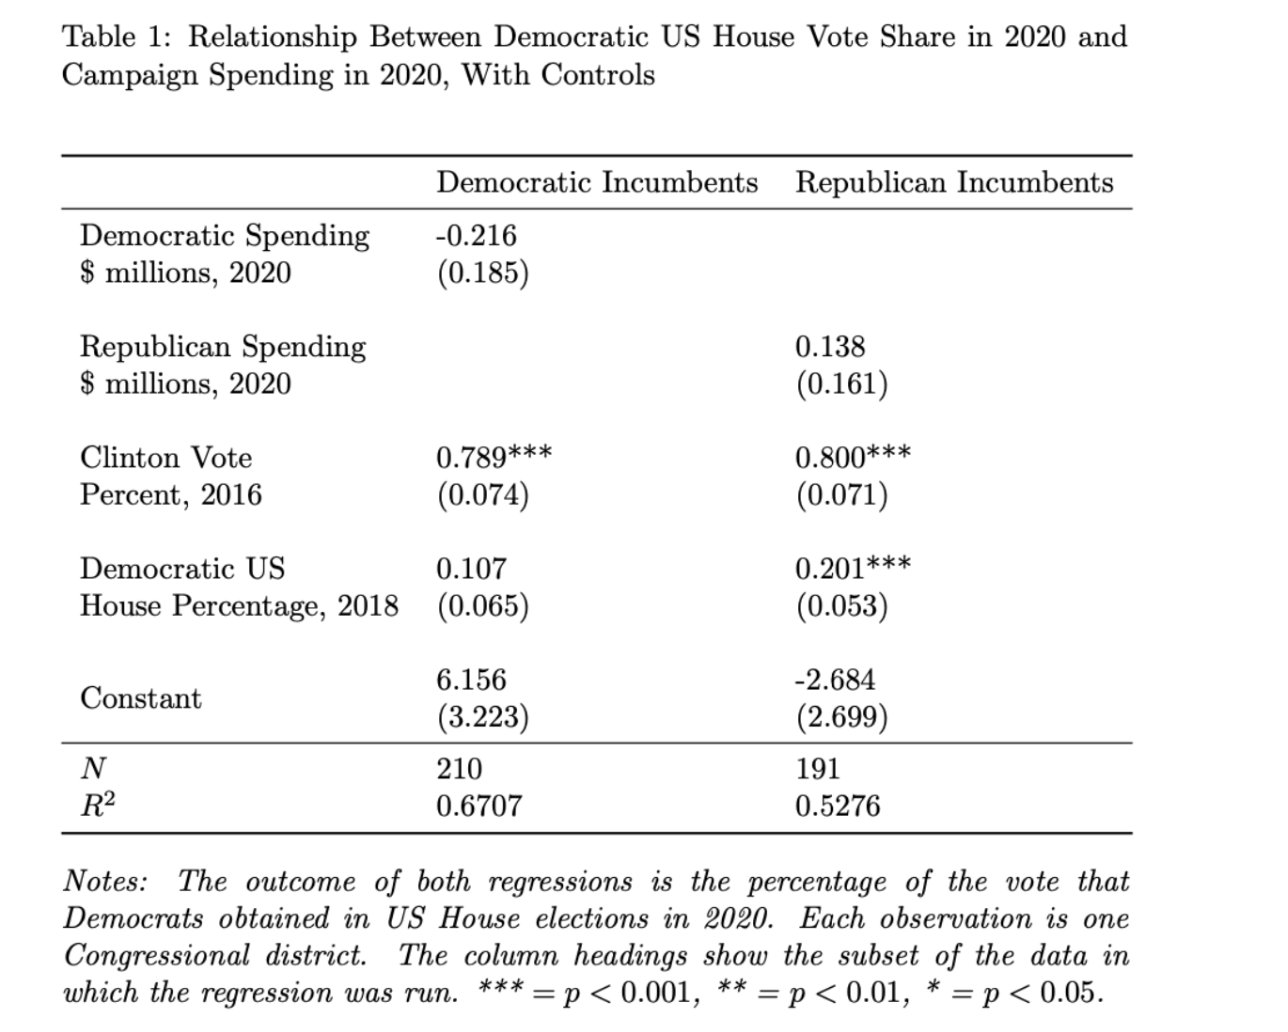
\includegraphics[width=\textwidth,height=0.78\textheight,keepaspectratio]{images/regression-table.png}};\begin{scope}[x={(img.south east)},y={(img.north west)}]\draw[targetred,ultra thick,fill=targetred,fill opacity=0.15] (0.3283,{1-0.4159}) rectangle ({0.3283+0.0692},{1-0.4159-0.0511});\end{scope}\end{tikzpicture}\end{center}
\end{frame}

\begin{frame}{Table Walkthrough: Significance Stars}
\protect\phantomsection\label{table-walkthrough-significance-stars}
\begin{center}\begin{tikzpicture}\node[anchor=south west,inner sep=0] (img) at (0,0) {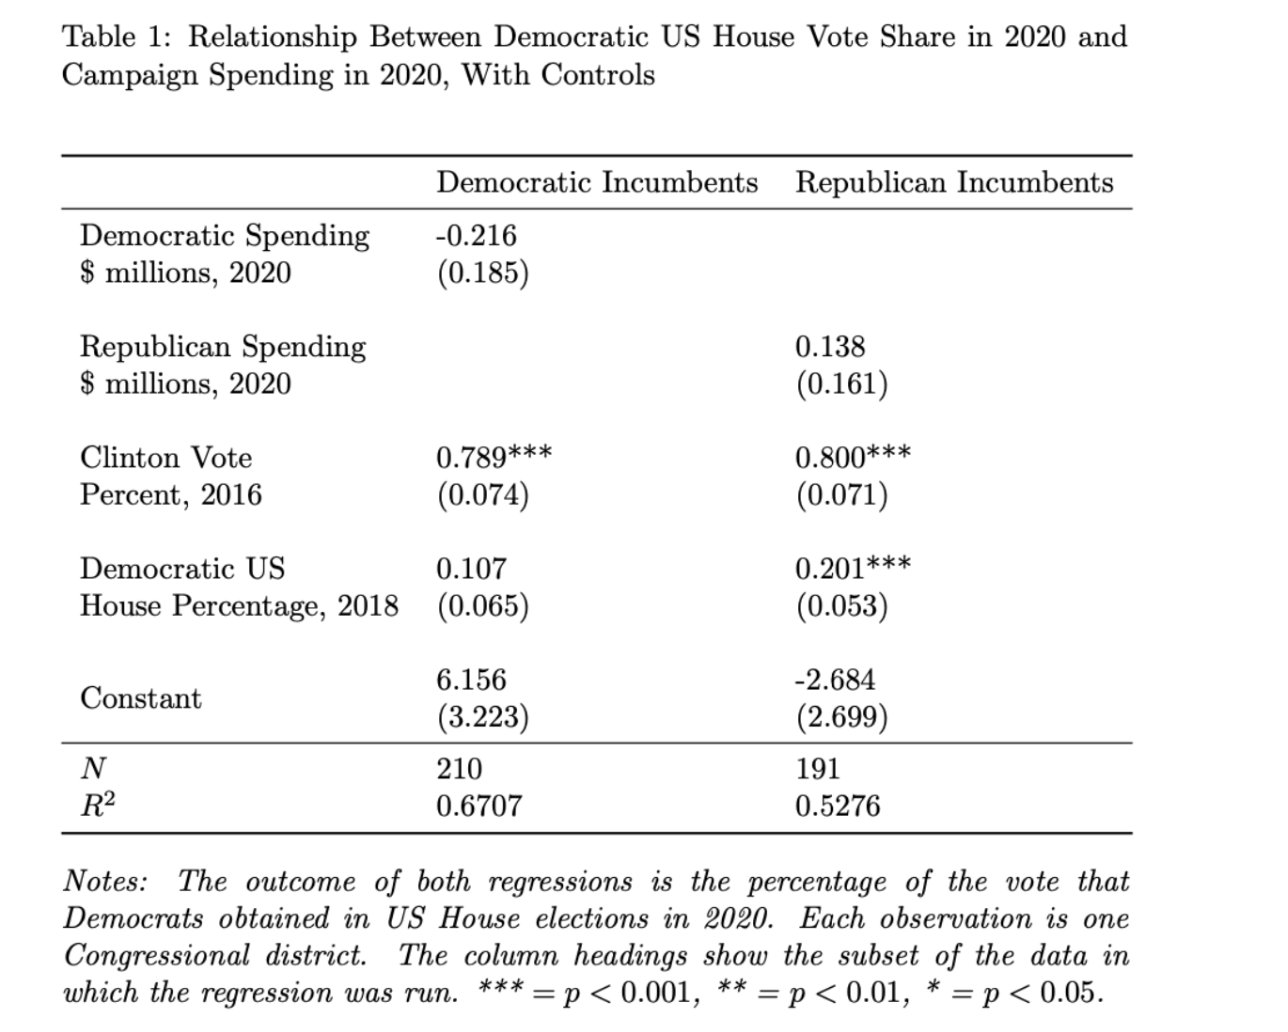
\includegraphics[width=\textwidth,height=0.78\textheight,keepaspectratio]{images/regression-table.png}};\begin{scope}[x={(img.south east)},y={(img.north west)}]\draw[targetred,ultra thick,fill=targetred,fill opacity=0.15] (0.3928,{1-0.4159}) rectangle ({0.3928+0.0441},{1-0.4159-0.0412});\end{scope}\end{tikzpicture}\end{center}
\end{frame}

\begin{frame}{Example}
\protect\phantomsection\label{example}
\small

Top-left box of the previous table:

\begin{enumerate}
\tightlist
\item
  Based on the title, it seems that we're supposed to look at how
  Democratic spending is related to Democratic vote share in 2020
  Congressional races. ``Controls'' implies a multiple linear
  regression. \pause
\item
  The model is called ``Democratic incumbents''. The outcome is the vote
  share for Democrats in 2020 Congressional races, but only in races
  where Democrats already held the seat. \pause
\item
  The row refers to Democratic spending in 2020 and should be
  interpreted in millions of dollars. \pause
\item
  Given that ``vote share'' is in percentage points, and Democratic
  spending is in millions of dollars: an increase of \$1 million dollars
  in Democratic spending is associated with, on average, a 0.22\%
  decrease in Democratic vote share in 2020 Congressional races where
  Democrats were the incumbents. \pause
\item
  This relationship is not significant (note that the standard error and
  estimate are of similar size!) \pause

  \begin{enumerate}
  [a.]
  \tightlist
  \item
    \textbf{None of these variables have a causal interpretation because
    the variables are not randomly assigned.}
  \end{enumerate}
\end{enumerate}

\normalsize
\end{frame}

\begin{frame}{PS 3: Week 13}
\protect\phantomsection\label{ps-3-week-13}
\vspace{1.2cm}
\begin{center}
\Large Natural Experiments
\end{center}
\end{frame}

\begin{frame}{Agenda}
\protect\phantomsection\label{agenda-1}
\begin{enumerate}
\tightlist
\item
  Attendance Survey
\item
  Reviewing Regression Tables
\item
  Natural Experiments
\item
  Instrumental Variables
\item
  Example of Instrumental Variables
\end{enumerate}
\end{frame}

\begin{frame}{Housekeeping}
\protect\phantomsection\label{housekeeping}
\begin{itemize}
\tightlist
\item
  First Draft of Report due 11/21 \pause

  \begin{itemize}
  \tightlist
  \item
    You can look at results as a group \pause
  \item
    \textbf{Write the reports individually} \pause

    \begin{itemize}
    \tightlist
    \item
      Three statistical tests + interpretations \pause
    \end{itemize}
  \item
    Make sure you go to the instructions Google Doc and upload \pause
  \end{itemize}
\item
  Presentation due 11/26 (day before Thanksgiving) \pause

  \begin{itemize}
  \tightlist
  \item
    Upload slides on bCourses \pause
  \item
    5-7 minute presentations \pause
  \end{itemize}
\item
  We will hold presentations the last day of section \pause

  \begin{itemize}
  \tightlist
  \item
    Because of this, next week will be some final review!
  \end{itemize}
\end{itemize}
\end{frame}

\section{Review of Regression Tables}\label{review-of-regression-tables}

\begin{frame}{Interpreting a Regression Table}
\protect\phantomsection\label{interpreting-a-regression-table}
\small

\begin{enumerate}
\tightlist
\item
  Look at the \textbf{title} of the table \pause

  \begin{enumerate}
  [a.]
  \tightlist
  \item
    \textcolor{blue}{What are the authors generally trying to tell us?}
  \item
    This can clue you into relevant variables and takeaways, though keep
    a critical eye to the table yourself! \pause
  \end{enumerate}
\item
  Look at the title of each \textbf{column} (this is the title of each
  regression model) \pause

  \begin{enumerate}
  [a.]
  \tightlist
  \item
    \textcolor{blue}{What is each model trying to tell me? What subset of data are they using? What outcome?}
    \pause
  \end{enumerate}
\item
  Look at the \textbf{row} labels (these are the predictor variables)
  \pause

  \begin{enumerate}
  [a.]
  \tightlist
  \item
    \textcolor{blue}{Which ones are causal (treatment assignment)? Which ones are not (any other variables)?}
    \pause
  \end{enumerate}
\item
  Look at the point \textbf{estimates} themselves \pause

  \begin{enumerate}
  [a.]
  \tightlist
  \item
    \textcolor{blue}{Based on the row label and column title, what is this estimate telling me?}
    \pause
  \end{enumerate}
\item
  Look at the measures of \textbf{noise} \pause

  \begin{enumerate}
  [a.]
  \tightlist
  \item
    \textcolor{blue}{Is the estimate significant? How do I interpret significance in this context?}

    \begin{enumerate}
    [i.]
    \tightlist
    \item
      \textcolor{blue}{Is it causal?}
    \end{enumerate}
  \end{enumerate}
\end{enumerate}

\normalsize
\end{frame}

\begin{frame}{Regression Table Example}
\protect\phantomsection\label{regression-table-example}
\begin{center}\begin{tikzpicture}\node[anchor=south west,inner sep=0] (img) at (0,0) {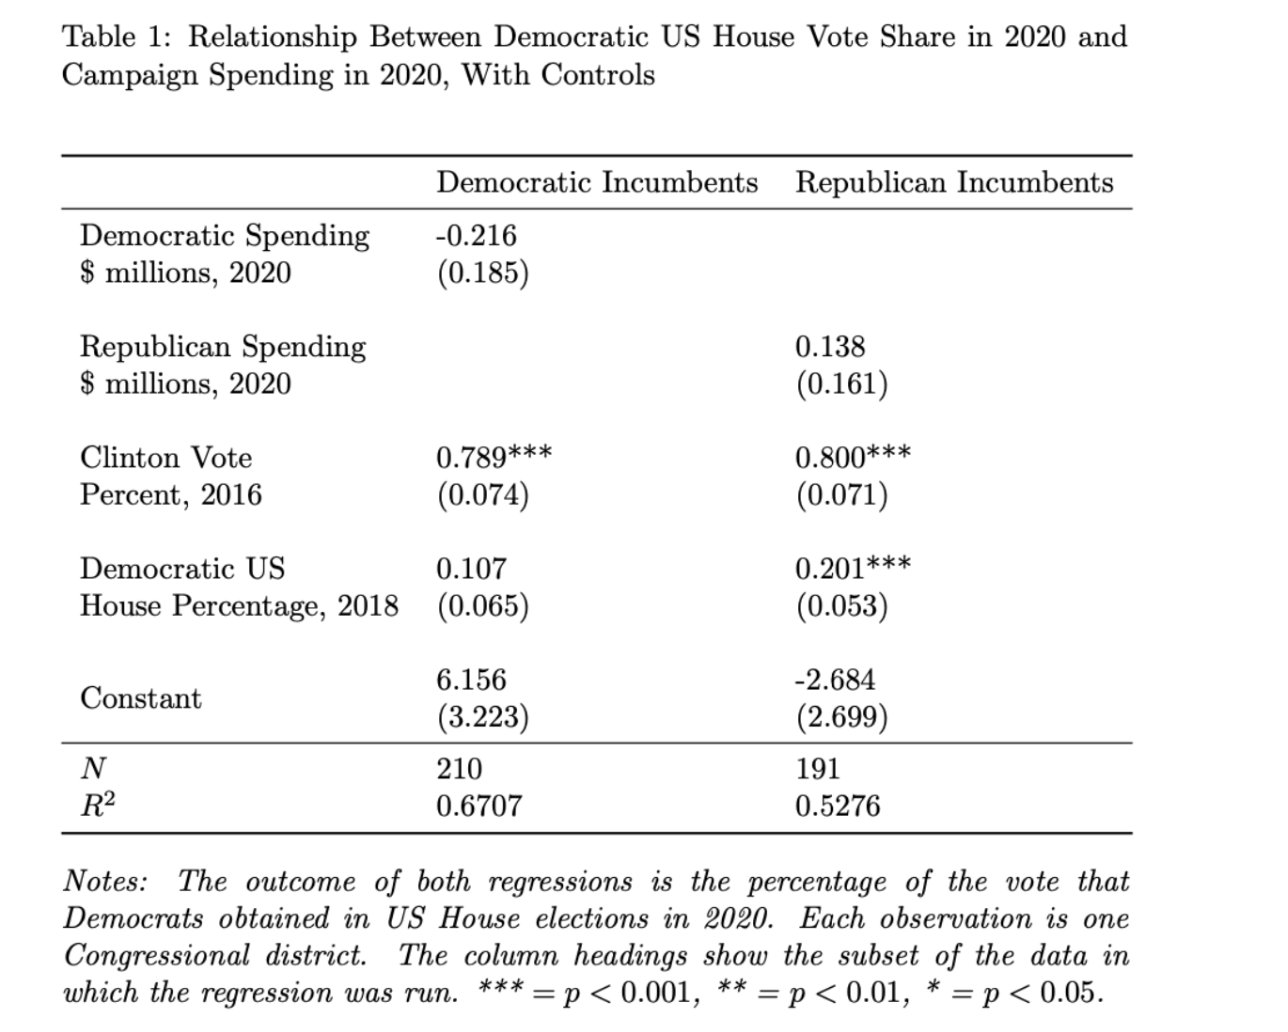
\includegraphics[width=\textwidth,height=0.78\textheight,keepaspectratio]{images/regression-table.png}};\begin{scope}[x={(img.south east)},y={(img.north west)}]\draw[targetred,ultra thick,fill=targetred,fill opacity=0.15] (0.3205,{1-0.2115}) rectangle ({0.3205+0.1038},{1-0.2115-0.0845});\end{scope}\end{tikzpicture}\end{center}
\end{frame}

\begin{frame}{Example}
\protect\phantomsection\label{example-1}
\small

Top-left box of the previous table:

\begin{enumerate}
\tightlist
\item
  Based on the title, it seems that we're supposed to look at how
  Democratic spending is related to Democratic vote share in 2020
  Congressional races. ``Controls'' implies a multiple linear
  regression. \pause
\item
  The model is called ``Democratic incumbents''. The outcome is the vote
  share for Democrats in 2020 Congressional races, but only in races
  where Democrats already held the seat. \pause
\item
  The row refers to Democratic spending in 2020 and should be
  interpreted in millions of dollars. \pause
\item
  Given that ``vote share'' is in percentage points, and Democratic
  spending is in millions of dollars: an increase of \$1 million dollars
  in Democratic spending is associated with, on average, a 0.22\%
  decrease in Democratic vote share in 2020 Congressional races where
  Democrats were the incumbents. \pause
\item
  This relationship is not significant (note that the standard error and
  estimate are of similar size!) \pause

  \begin{enumerate}
  [a.]
  \tightlist
  \item
    \textbf{None of these variables have a causal interpretation because
    the variables are not randomly assigned.}
  \end{enumerate}
\end{enumerate}

\normalsize
\end{frame}

\section{Natural Experiments}\label{natural-experiments}

\begin{frame}{The Revenge of Observational Data}
\protect\phantomsection\label{the-revenge-of-observational-data}
\begin{itemize}
\tightlist
\item
  We know randomized experiments have many benefits---by randomly
  assigning treatment, we can estimate a causal effect by eliminating
  various sources of bias \pause
\item
  But they also have limitations---you are viewing an effect in one
  study at one point in time, tested on one sample. \pause
\item
  Observational data has many benefits---it's real-world data that can
  more convincingly generalize to real-world processes \pause
\item
  But we rarely see a randomization of
  treatment---\textcolor{blue}{can we identify a causal effect?}
\end{itemize}
\end{frame}

\begin{frame}{Natural Experiments}
\protect\phantomsection\label{natural-experiments-1}
\begin{itemize}
\tightlist
\item
  We can find randomization in the real-world to take advantage of the
  benefits of both real-world data and randomization of treatment \pause
\item
  Examples \pause

  \begin{itemize}
  \tightlist
  \item
    Having a son or daughter \pause
  \item
    Experiencing more (or less) rainfall \pause
  \item
    Living on one Greek island instead of another \pause
  \item
    Being drafted (Vietnam war) \pause
  \item
    Barely winning (vs.~losing) an election \pause
  \end{itemize}
\item
  In all these cases, you have to make the case that randomization is
  actually occurring \pause
\item
  We don't control randomization, but we claim that we found it
\end{itemize}
\end{frame}

\section{Instrumental Variables}\label{instrumental-variables}

\begin{frame}{Instrumental Variables}
\protect\phantomsection\label{instrumental-variables-1}
\begin{itemize}
\tightlist
\item
  Say we want to know if X causes Y, but X is not randomly assigned.
  \textcolor{blue}{What do we do?} \pause
\item
  If we find something that is random that causes X, we can argue for
  as-if randomization \pause

  \begin{itemize}
  \tightlist
  \item
    This is called an \textbf{instrument} \pause
  \item
    The instrument is what performs the random assignment of X (our
    hypothetical treatment)
  \end{itemize}
\end{itemize}
\end{frame}

\begin{frame}{An Example: Military Service}
\protect\phantomsection\label{an-example-military-service}
\begin{center}
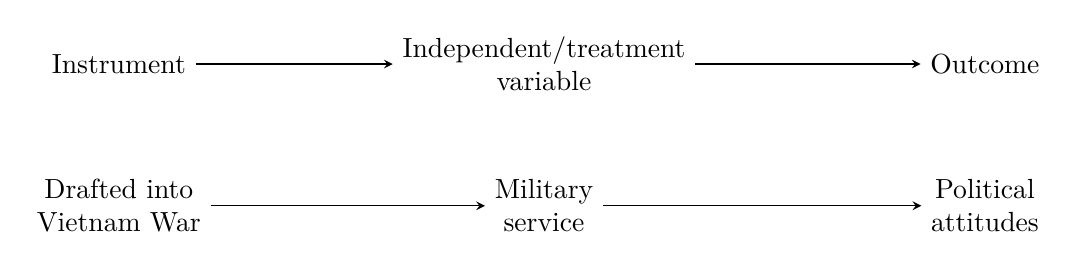
\begin{tikzpicture}[>=stealth, every node/.style={align=center}]
\node (i1) at (0,1.8) {Instrument};
\node (t1) at (5.4,1.8) {Independent/treatment\\variable};
\node (o1) at (11,1.8) {Outcome};
\draw[->] (i1) -- (t1);
\draw[->] (t1) -- (o1);
\node<2-> (i2) at (0,0) {Drafted into\\Vietnam War};
\node<2-> (t2) at (5.4,0) {Military\\service};
\node<2-> (o2) at (11,0) {Political\\attitudes};
\draw<2->[->] (i2) -- (t2);
\draw<2->[->] (t2) -- (o2);
\end{tikzpicture}
\end{center}
\end{frame}

\begin{frame}{An Example: Military Service}
\protect\phantomsection\label{an-example-military-service-1}
\begin{center}
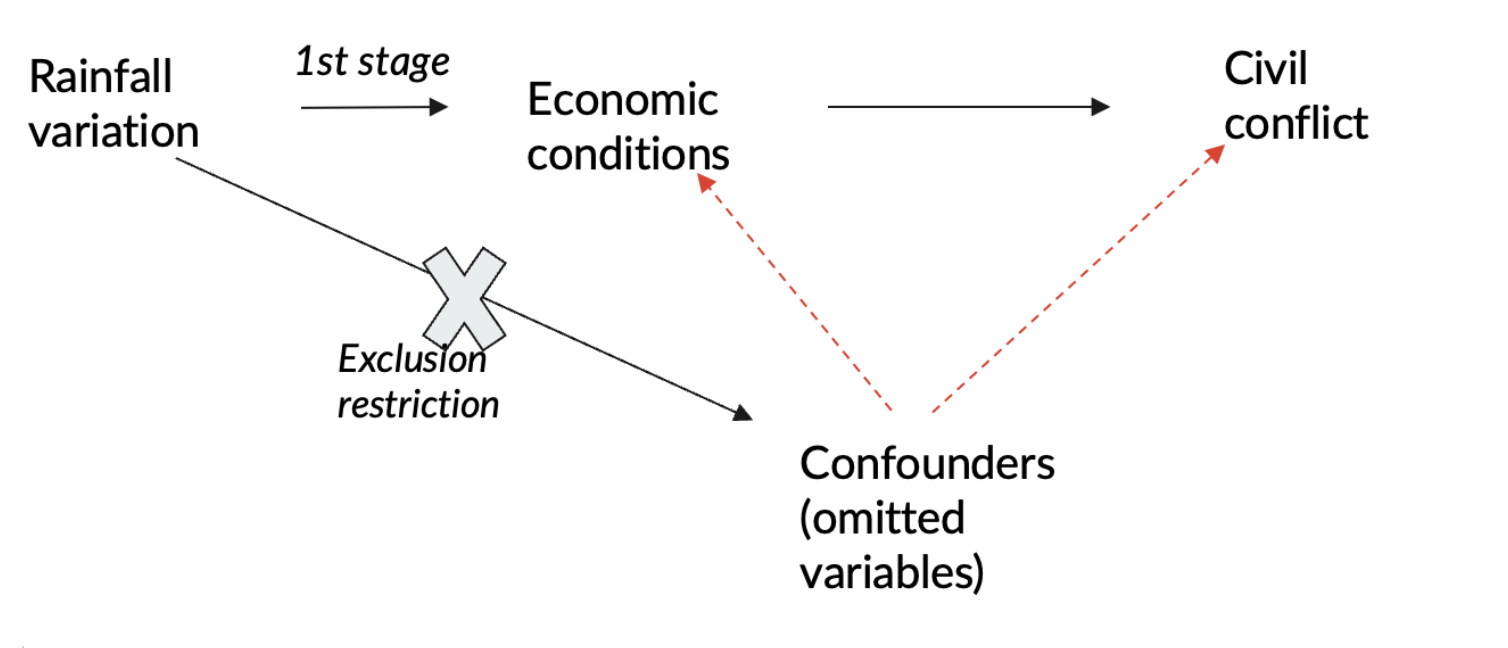
\includegraphics[height=0.42\textheight,alt={Diagram of an instrumental variable design. An arrow labeled first stage runs from the instrument to the independent variable, and another arrow runs from the independent variable to the outcome. Confounders (omitted variables) affect both the independent variable and the outcome, shown with dashed red arrows. A crossed-out arrow from the instrument directly to the outcome is labeled exclusion restriction.}]{images/iv-diagram.png}
\end{center}

\small

Requirements: \pause

\begin{enumerate}
\tightlist
\item
  Instrument is randomly assigned \pause
\item
  \textbf{First-Stage Condition}: Instrument must be correlated with X
  \pause
\item
  \textbf{Exclusion Restriction}: Instrument affects the y
  \underline{only through our x} \pause
\end{enumerate}

If these requirements are met, we can compare those who receive the
instrument to those who do not to estimate a causal effect.

\normalsize
\end{frame}

\begin{frame}{An Example: Military Service}
\protect\phantomsection\label{an-example-military-service-2}
\begin{center}
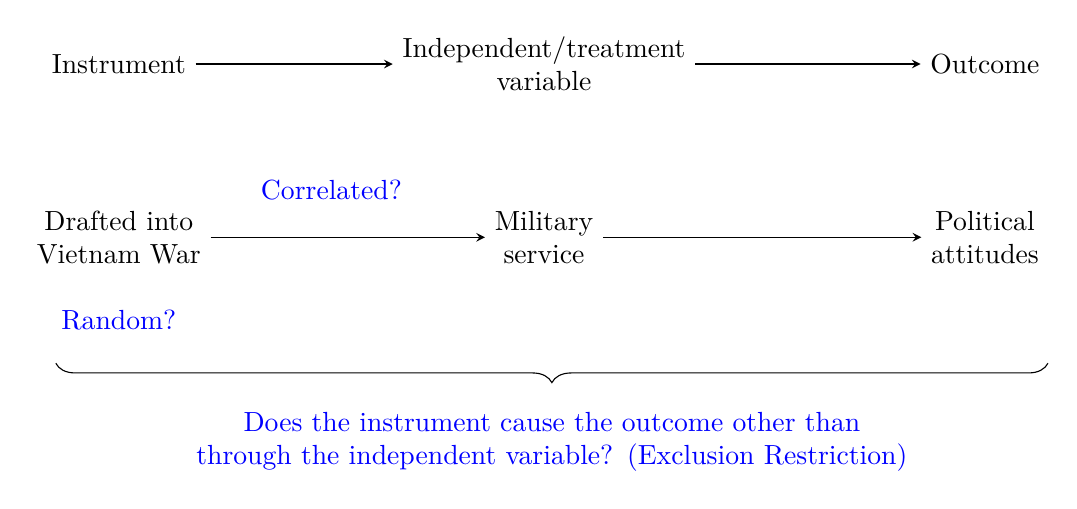
\begin{tikzpicture}[>=stealth, every node/.style={align=center}]
\node (i1) at (0,2.2) {Instrument};
\node (t1) at (5.4,2.2) {Independent/treatment\\variable};
\node (o1) at (11,2.2) {Outcome};
\draw[->] (i1) -- (t1);
\draw[->] (t1) -- (o1);
\node (i2) at (0,0) {Drafted into\\Vietnam War};
\node (t2) at (5.4,0) {Military\\service};
\node (o2) at (11,0) {Political\\attitudes};
\draw[->] (i2) -- (t2);
\draw[->] (t2) -- (o2);
\node<2->[text=blue] at (2.7,0.6) {Correlated?};
\node<3->[text=blue] at (0,-1.05) {Random?};
\draw<4->[decorate,decoration={brace,mirror,amplitude=7pt}] (-0.8,-1.6) -- (11.8,-1.6);
\node<4->[text=blue,text width=11.5cm] at (5.5,-2.6) {\hyphenpenalty=10000 Does the instrument cause the outcome other than through the independent variable? (Exclusion Restriction)};
\end{tikzpicture}
\end{center}
\end{frame}

\section{Instrumental Variables: An
Example}\label{instrumental-variables-an-example}

\begin{frame}{Paper: Economic Shocks and Civil Conflict}
\protect\phantomsection\label{paper-economic-shocks-and-civil-conflict}
\begin{center}

\includegraphics[height=0.7\textheight,alt={Abstract of the paper Economic Shocks and Civil Conflict: An Instrumental Variables Approach, by Edward Miguel, Shanker Satyanath, and Ernest Sergenti. The authors use rainfall variation as an instrumental variable for economic conditions in 41 African countries during 1981 to 1999, and find that negative growth shocks increase the likelihood of civil conflict.}]{images/miguel-paper-abstract.png}

Paper link: \url{https://www.journals.uchicago.edu/doi/10.1086/421174}
\end{center}
\end{frame}

\begin{frame}{Discussion Questions}
\protect\phantomsection\label{discussion-questions}
\begin{itemize}
\tightlist
\item
  \textcolor{blue}{1: What is the outcome variable?}
\item
  \textcolor{blue}{2: What is the independent/treatment variable?}
\item
  \textcolor{blue}{3: What is the instrument?}
\item
  \textcolor{blue}{4: Does the exclusion restriction hold? Why might it not hold?}
\end{itemize}

\pause

Discuss with your neighbors for 10 min and we will share answers
together.
\end{frame}

\begin{frame}{Answers: Rainfall as an Instrument}
\protect\phantomsection\label{answers-rainfall-as-an-instrument}
\begin{center}
\includegraphics[height=0.75\textheight,alt={Instrumental variable diagram for the paper. Rainfall variation has a first-stage arrow to economic conditions, which has an arrow to civil conflict. Confounders (omitted variables) affect both economic conditions and civil conflict, shown with dashed red arrows. A crossed-out arrow from rainfall variation directly to civil conflict is labeled exclusion restriction.}]{images/rainfall-diagram.png}
\end{center}
\end{frame}

\begin{frame}{Acknowledgements}
\protect\phantomsection\label{acknowledgements}
Special thanks to prior GSIs for providing materials off of which some
of these slides are based, especially Will Halm.
\end{frame}

\end{document}
